\documentclass{beamer}
\usepackage[utf8]{inputenc}

\usetheme{Madrid}
\usecolortheme{default}
\usepackage{amsmath,amssymb,amsfonts,amsthm}
\usepackage{txfonts}
\usepackage{tkz-euclide}
\usepackage{listings}
\usepackage{adjustbox}
\usepackage{array}
\usepackage{tabularx}
\usepackage{gvv}
\usepackage{lmodern}
\usepackage{circuitikz}
\usepackage{tikz}
\usepackage{graphicx}

\setbeamertemplate{page number in head/foot}[totalframenumber]

\usepackage{tcolorbox}
\tcbuselibrary{minted,breakable,xparse,skins}



\definecolor{bg}{gray}{0.95}
\DeclareTCBListing{mintedbox}{O{}m!O{}}{%
  breakable=true,
  listing engine=minted,
  listing only,
  minted language=#2,
  minted style=default,
  minted options={%
    linenos,
    gobble=0,
    breaklines=true,
    breakafter=,,
    fontsize=\small,
    numbersep=8pt,
    #1},
  boxsep=0pt,
  left skip=0pt,
  right skip=0pt,
  left=25pt,
  right=0pt,
  top=3pt,
  bottom=3pt,
  arc=5pt,
  leftrule=0pt,
  rightrule=0pt,
  bottomrule=2pt,
  toprule=2pt,
  colback=bg,
  colframe=orange!70,
  enhanced,
  overlay={%
    \begin{tcbclipinterior}
    \fill[orange!20!white] (frame.south west) rectangle ([xshift=20pt]frame.north west);
    \end{tcbclipinterior}},
  #3,
}
\lstset{
    language=C,
    basicstyle=\ttfamily\small,
    keywordstyle=\color{blue},
    stringstyle=\color{orange},
    commentstyle=\color{green!60!black},
    numbers=left,
    numberstyle=\tiny\color{gray},
    breaklines=true,
    showstringspaces=false,
}
%------------------------------------------------------------

\title
{4.12.8}
\date{September 11,2025}
\author 
{AI25BTECH11003 - Bhavesh Gaikwad}



\begin{document}


\frame{\titlepage}
\begin{frame}{Question}
Distance of the point $(\alpha, \beta, \gamma)$ from y-axis is\\
a) $\beta$\\
b) $|\beta|$\\
c) $|\beta + \gamma|$\\
d)$\sqrt{\alpha^2 + \gamma^2}$ \\
\end{frame}


\begin{frame}[fragile]
    \frametitle{Theoretical Solution}
Let $\vec{A} = \myvec{\alpha \\ \beta \\ \gamma}$\\
Let $\vec{B}$ be the point on y-axis which is nearest to $\vec{A}$.\\


\begin{equation}
\text{Equation of y-axis: } \vec{r} = \lambda \vec{e_2}, \, where \, e_2=\myvec{0 \\ 1 \\ 0}
\end{equation}


Since point $\vec{B}$ satisfies the equation,
\begin{equation}
    \vec{B} = \lambda \vec{e_2}
\end{equation}
\end{frame}

\begin{frame}[fragile]
    \frametitle{Theoretical Solution}
$\vec{(B-A)}$ is perpendicular to the y-axis as its the shortest distance between a line and a point $\vec{A}$ or $\vec{B-A}$ is perpendicular to $\vec{B}$ as it lies on the y-axis itself.

\begin{equation}
    \therefore \, \vec{(B-A)}^\top\vec{B} = 0
\end{equation}

\begin{equation}
    \vec{A}^\top\vec{B} - \norm{\vec{B}}^2 = 0 \, \, \Rightarrow \, \,
    \vec{A}^\top\vec{B} = \norm{\vec{B}}^2
\end{equation}

From Equations 2 and 4,
\begin{equation}
    \vec{A}^\top (\lambda\vec{e_2})=\lambda^2
\end{equation}

\begin{equation}
    \therefore \, \lambda = \vec{e_2}^\top\vec{A} \quad \Rightarrow
    \lambda = \beta 
\end{equation}

From Equation 6,
\begin{equation}
    \vec{B} = \beta\vec{e_2} \, \, OR \, \, \vec{B} = \beta\myvec{0 \\ 1 \\ 0}
\end{equation}
\end{frame}

\begin{frame}[fragile]
    \frametitle{Theoretical Solution}
Let d be the shortest distance between the y-axis and $\vec{A}$.

\begin{equation}
    d = \norm{\vec{B}-\vec{A}} = \sqrt{\vec{(B-A)}^\top\vec{(B-A)}} \,  
\end{equation}

\begin{equation}
\therefore \, d = \sqrt{\alpha^2 + \gamma^2}    
\end{equation}

\begin{center}
$\boxed{\text{Therefore, Option D is Correct.}}$
\end{center}
\end{frame}

\begin{frame}{Image}
\begin{figure}
   \centering
    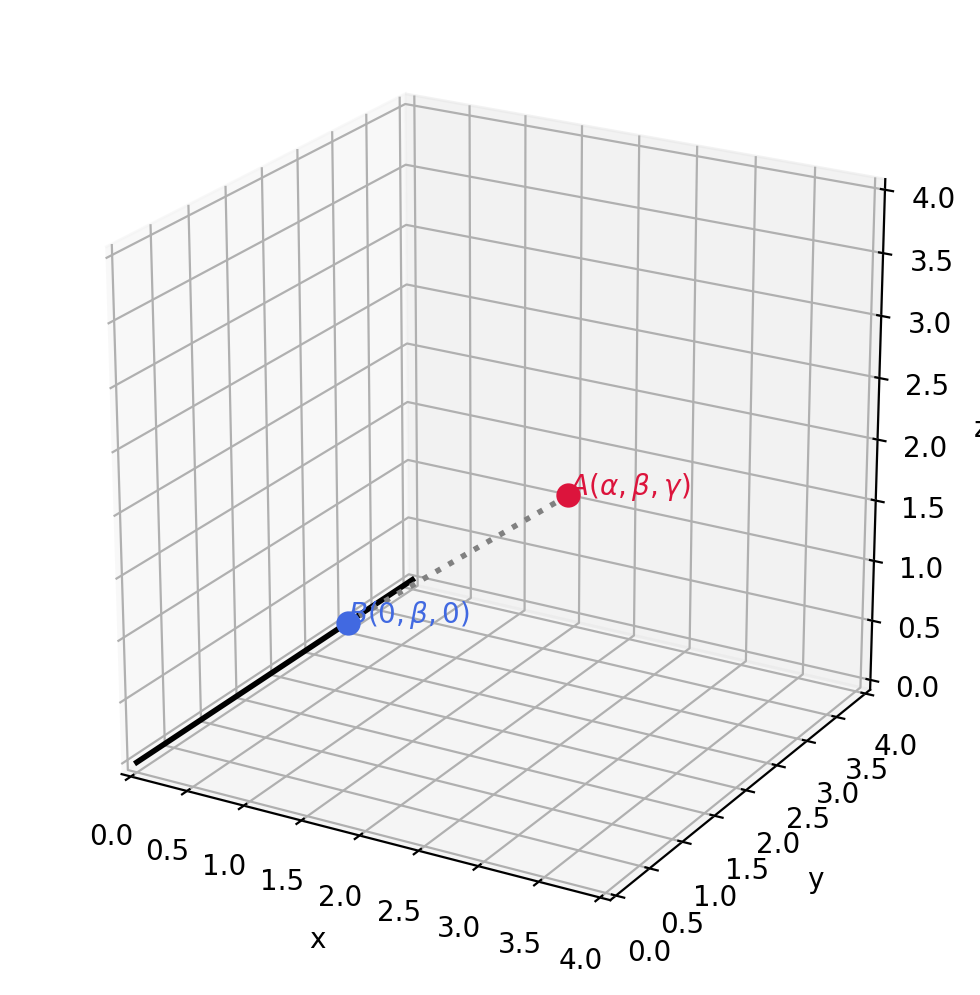
\includegraphics[width=\columnwidth, height=0.8\textheight, keepaspectratio]{figs/fig1.png}
    \label{fig:Beamer/figs/fig1.png}
\end{figure}
\end{frame}


\end{document}